\documentclass[onecolumn,draftclsnofoot, 10pt, compsoc]{IEEEtran}

\usepackage{graphicx}
\usepackage[section]{placeins}
\usepackage{caption}

\usepackage{amssymb}                                         
\usepackage{amsmath}                                         
\usepackage{amsthm}                                

\usepackage{alltt}                                           
\usepackage{float}
\usepackage{color}
\usepackage{url}

\usepackage{balance}
\usepackage[TABBOTCAP, tight]{subfigure}
\usepackage{enumitem}
\usepackage{pstricks, pst-node}
\usepackage{url}
\usepackage{setspace}

\usepackage{etoolbox}
\AtBeginEnvironment{quote}{\singlespacing\vspace{-\topsep}\small}

%\input{pygments.tex}

\usepackage{geometry}
\geometry{left=0.75in,right=0.75in,top=0.75in,bottom=0.75in}
\parindent = 0.0 in
\parskip = 0.1 in


\def \ParSpace{\vspace{.75em}}
\def \GroupNumber{		17}
\def \Jeremy{			Jeremy Fischer}
\def \Class{		Operating Systems ii}
\def \School{	Oregon State University}
\def \Professor{		 Kevin McGrath}

\newcommand{\cred}[1]{{\color{red}#1}}
\newcommand{\cblue}[1]{{\color{blue}#1}}

\newcommand{\NameSigPair}[1]{
		\par
		\makebox[2.75in][r]{#1} \hfil 	\makebox[3.25in]{\makebox[2.25in]{\hrulefill} \hfill			
		\makebox[.75in]{\hrulefill}}
		\par\vspace{-12pt} \textit{
			\tiny\noindent
			\makebox[2.75in]{} \hfil		
			\makebox[3.25in]{
				\makebox[2.25in][r]{Signature} \hfill	\makebox[.75in][r]{Date}
			}
		}
}










%%%%%%%%%%%%%%%%%%%%%%%%%%%%%%%%%%%%%%%
\begin{document}
\begin{titlepage}
    \pagenumbering{gobble}
    \begin{singlespace}
    	
\includegraphics[height=4cm]{coe.eps}
        \hfill  
        \par\vspace{.2in}
        \centering
        \scshape{
            \vspace{.5in}
            \textbf{\Huge\Class}\par
            \large{
            	\today \\Fall Term
        	}
            \vfill
            {\large Prepared for}\par
            \huge \School\par
            \vspace{5pt}
            {\Large{\Professor}\par}
            {\large Prepared by }\par
           % Group\GroupNumber\par
            \vspace{5pt}
            {\Large
                {\Jeremy}\par
            }
            \vspace{20pt}
        }
        \begin{abstract}
        	This document explores processes, threads, and CPU scheduling in the Linux, Windows, and FreeBSD operating systems. Followed is a comparison of the three.
        \end{abstract}     
    \end{singlespace}
\end{titlepage}
\newpage
\pagenumbering{arabic}
\tableofcontents
% 7. uncomment this (if applicable). Consider adding a page break.
%\listoffigures
%\listoftables
\clearpage









\section{Linux Implementation}


\subsection{Processes}
	Each process has its own private resources, data, and associated statistics about itself so the OS can make good scheduling decisions. 
	In memory the process is divided into segments: Stack, Heap, and Text. Program code is converted into machine readable instructions and is stored in the Text segment. 
	Local function-variables that are automatically allocated go in the Stack. 
	And memory dynamically allocated by the program go in the Heap. 
	As memory is used by a process the stack and heap grow toward each other. 
	If a process has shared libraries then it is mapped into process memory which is placed between the stack and the heap.
	A process can either be independent or cooperating \cite{processesLinux}.
	\begin{itemize}
		\item An independent process cannot affect or be affected by the execution of another process
		\item Cooperating processes can affect or be affected by another process. This is usually done for information sharing
	\end{itemize}

	\ParSpace
	Each process has information associated to itself so the operating system can achieve certain tasks efficiently.  The operating system tracks\dots
	\begin{itemize}
		\item The memory the process is using as well as where in the memory the process is currently executing (instruction pointer)
		\item Any open files or network connections the process is using
		\item The amount of CPU time a process has used as well as the amount of RAM being consumed by the process
		\item Each process has a process ID so the OS can distinguish it from other processes. 
		\item The current process's parent i.e. the process that created the current process. This is done so the OS can handle permissions to resources efficiently
	\end{itemize}
	
	\ParSpace
	All processes are created from a parent process, except for the \textbf{init} process with is created by the OS kernel. 
	 All other processes are a child of \textbf{init}  (parent of all parents).
	 The \textbf{init}  process must remain alive for the entire time the system is up and running.
	 The \textbf{init} process has a process ID of 1. 
	 A process is created by its parent making a copy of itself - called forking.
	 The child's memory space is initially an exact copy of its parent.
	 The parent however, decides which resources to share with its child. Resources such as open file descriptors and open network connections are shared by default. The parent may decided not to share any resources, making the forked process independent.
	 Once a child is initialized it is its own process that can run in parallel with the parent. 
	 The parent can either wait on the child to finish doing its work before continuing, or it can continue on its own duties, or it can kill the child process.
	 A child process can load a completely different program into its allocated memory, which replaces the copy of the parents program. This is called "exec-ing" due to it being done through the \textit{exec} command. 
	 
 

\subsection{Threads}
	A thread can be thought of as a light weight process. 
	As in, there's no need to allocate memory for the thread. 
	The thread instead shares the memory of the process that it is in (except the stack segment).
	Linux threads follow a co-operative multitasking scheme where the threads are executed sequentially. 
	However, the time to switch from one thread to the next is so incredibly fast that it appears they're running in parallel. 
	The downside to this scheme is that if one thread gets blocked then the whole process gets blocked \cite{threadsVidLinux}.
	Each thread is dependent on the process and other threads. They all share the same data. A thread can only access data within its process.
	Processes are the entities that group resources together. Threads are the entities that are actually scheduled for execution by the CPU.
	There are user threads and kernel threads \cite{threadsArtiLinux}:
	\begin{itemize}
		\item User threads are created and killed in user space. 
		The kernel is not aware of these threads, meaning it is not involved in their processing.
		\item Kernel threads are created and killed by the kernel. 
		Each thread that exists in the user space has a counterpart kernel thread. 
		Since these threads are managed by the kernel they follow preemptive multitasking - meaning the scheduler can stop a thread's execution so a higher priority thread can run. 
		In contrast to user threads, if a kernel thread gets blocked it doesn't cause the whole system to block since it follows a preemptive scheduling model. 
		However, switching from one thread to the next is slower for kernel threads.
		
	\end{itemize}
	
\subsection{CPU Scheduling}
	The Completely Fair Scheduler, CFS, is a task scheduler that Linux introduced in version 2.6.23 \cite{schedulerLinux}. 
	Its goal is to utilize the CPU as efficiently as possible by handling resource allocation. 
	The scheduler uses red-black trees instead of run queues like Windows.
	The main idea is to have the tree remain balanced, providing a fair amount of processing time to each process relative to the others. 
	When a process isn't given a fair amount then they are given extra time to execute.
	The CFS maintains the amount of time provided to a given task in the virtual runtime. 
	The smaller a task's virtual runtime, i.e. the smaller amount of assigned processor time, the higher its priority. 
	The CFS also includes the concept of sleeper fairness to ensure that tasks that are not currently runnable (waiting for I/O, etc.) receive a fair share of the processor when they eventually need it \cite{schedulerLinux}.


\section{Windows Implementation}

\subsection{Processes}

	\begin{figure}[H]
		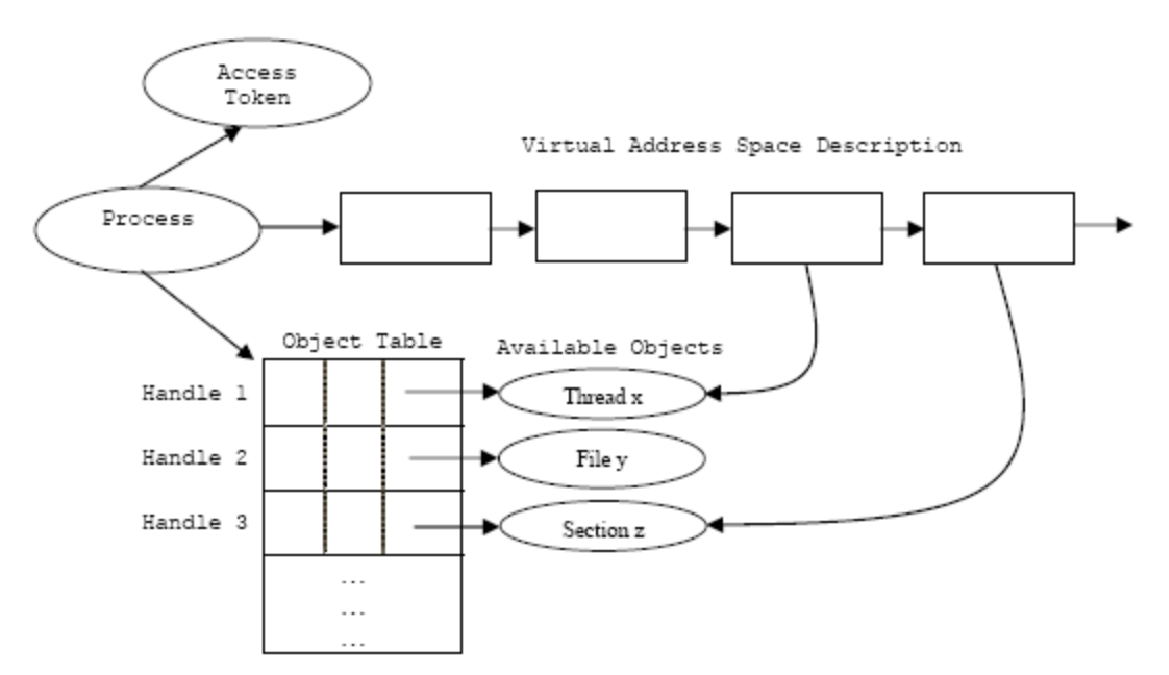
\includegraphics[width=.6\textwidth]{windowsProcessTemplate.eps}
		\centering
		\caption{Windows process object template used when creating a new process object \cite{windowsProcessMSDN}}
		\label{fig:mesh1}
	\end{figure}

	A Windows process has a virtual address space, executable code, open handles to system objects, a security context, a unique process identifier, environment variables, a priority class, minimum and maximum working set sizes, and at least one thread of execution \cite{windowsProcessMSDN}.
	Each process is represented as an object.
	When Windows creates a new process it uses the template outlined in figure \ref{fig:mesh1} to generate a new object instance. 
	The access token attached to each process lets the operating system know what the process has access to.
	When a process object is first created it is given an initial thread.
	This thread is refereed to as the \textit{primary thread}.
	Although a process starts with only one thread, each thread is capable of creating new ones.
	
\subsection{Threads}
	 A thread is the entity within a process that can be scheduled for execution. 
	 All threads of a process share the virtual address space and system resources pertaining to its encompassing process. In addition, each thread maintains exception handlers, a scheduling priority, thread local storage, a unique thread identifier, and a set of structures the system will use to save the thread context until it is scheduled. The thread context includes the thread's set of machine registers, the kernel stack, a thread environment block, and a user stack in the address space of the thread's process. \cite{windowsProcessMSDN}.
	Threads are ranked in a priority based system. 
	There are 33 priority levels - zero is the lowest and 32 is the highest. 
	However, only the zero-page thread can obtain a priority level of zero (The zero-page thread is a system thread responsible for zeroing any free pages when there are no other threads that need to run.).
	The threads are prioritized by two general rules:
	\begin{itemize}
		\item The priority class of its process
		\item The priority level of the thread within the priority class of its process
	\end{itemize}
	
	
\subsection{CPU Scheduling}
	The system treats all threads with the same priority as equal - i.e. there is no further favoring of threads then their priority level.
	All high priority threads are assigned a time-slice in a round-robin fashion. 
	In cases where no high priority threads are able to run (they're waiting), then time-slices are assigned to the next highest priority level of threads in the same round-robin fashion.
	When a higher priority thread stops waiting and is able to run, the system abruptly halts the lower priority threads, and assigns a full time-slice to the awakened higher priority thread.
	Windows maintains a queue of readily executable threads for each priority level \cite{windowsCSwitchesMSDN}.
	When a processor becomes available the following steps are taken by the system to allow the next thread to run:
	\begin{enumerate}
		\item Save the context of the thread that just finished executing.
		\item Place the thread that just finished executing at the end of the queue for its priority.
		\item Find the highest priority queue that contains ready threads.
		\item Remove the thread at the head of the queue, load its context, and execute it.
	\end{enumerate}
	This scheduling design prioritizes short jobs and I/O bound processes. 
	Another important note is that all processes get their priority boosted after a wait event. However, processes waiting for user I/O get a larger priority boost than processes waiting on disk I/O \cite{schedulerWindows}. 
	
	


\section{FreeBSD Implementation}

\subsection{Processes}
	\begin{figure}[H]
		\includegraphics[width=.55\textwidth]{FreeBSDProcess.eps}
		\centering
		\caption{FreeBSD process structure \cite{freeBSDProcess}}
		\label{fig:mesh1}
	\end{figure}

	
	A FreeBSD process is a program in execution. The FreeBSD process structure is very similar to that of the Linux process structure described above. A process has an address space containing a mapping of its program’s object code and global variables. A process also has a bundle of kernel resources that include its credentials, signal state, and its descriptor array that gives it access to files, pipes, sockets, and devices. Each process has at least one and possibly many threads that execute its code. 
\subsection{Threads}
	Every thread running in a process has a corresponding kernel thread, with its own kernel stack that represents the user thread when it is executing in the kernel as a result of a system call, page fault, or signal delivery. Much like Linux threads described above, FreeBSD threads that are belong to the same process share resources.
	All threads that are runnable are assigned a scheduling priority and a CPU by the high-level scheduler that determines in which run queue they are placed. 

\subsection{CPU Scheduling}
	The default FreeBSD scheduler is the ULE scheduler.
	The ULE scheduler is broken into two parts: a low-level sections which runs frequently and a more complex high-level section which runs at most a few times per second.
	The low-level scheduler runs each time a thread blocks.
	To do scheduling efficiently it maintains a set of run queues per CPU that are organized from high priority to low.
	When a thread blocks, the low-level's only job is to find out which thread is the highest priority and replace it with the blocked thread. 
	The high-level scheduler is in charge of prioritizing each thread and figuring out which CPU's run queue a thread should be placed.
	 In selecting a new thread to run, the low-level scheduler scans the run queues of the CPU needing a new thread from highest to lowest priority and chooses the first thread on the first nonempty queue.
	 If there is more than one thread in the queue, the system runs them in a round robin fashion. 
	 That is, it runs them in a FIFO order, with equal amounts of CPU time. 
	 If a thread blocks, it is not put back onto a run queue. 
	 Instead, it is placed on a \textit{sleepqueue}. 
	 If a thread uses up the time slice allowed it, it is placed at the end of the queue from which it came, and the thread at the front of the queue is selected to run \cite{freeBSDScheduler}.
 

\section{Compare}
	The three operating systems are very similar as far as processes and threads go, especially Linux and FreeBSD. 
	The Linux scheduler, Completely Fair Scheduler, is most notably different from the Windows and FreeBSD schedulers in the way that threads are selected. 
	The CFS doesn't implement run queues. 
	Instead it keeps a red-black tree that is indexed by time spent on the CPU. 
	The reason for this is most likely because the red-black tree implements fairness with only an O(log N) overhead. 
	Another important difference between CFS and the other two schedulers according to Kernal Trap is that 
	
		\begin{quote}
			"CFS uses nanosecond granularity accounting and does not rely on any jiffies or other HZ detail. Thus the CFS scheduler has no notion of 'timeslices' and has no heuristics whatsoever. There is only one central tunable which can be used to tune the scheduler from 'desktop' (low latencies) to 'server' (good batching) workloads."\cite{CFSTimeSliceDifference}
		\end{quote}
	
	I think this difference makes Linux flexible. A user can simply change the granularity to a level that best suits their needs.
	Both Linux and FreeBSD keep parent-child relationships amongst threads and processes. Windows on the other hand does not. 
	Each thread is independent in nature. I think Windows left this relationship structure out so if a thread or process goes wrong the system can simply dispose of it without having to worry about handling the consequences that has on its parent or children.
	Linux doesn't differentiate much between a process and a thread. 
	Everything is simply a runnable task. 
	On the other hand, Windows differentiates the two pretty strongly. 
	A Windows process is an object, much like a container, that holds the resources that a thread needs. 
	The thread is what is actually scheduled to be placed on the CPU and does the work.
	
	
\bibliographystyle{IEEEtran}
\bibliography{references}

\end{document}